% Options for packages loaded elsewhere
\PassOptionsToPackage{unicode}{hyperref}
\PassOptionsToPackage{hyphens}{url}
%
\documentclass[
]{article}
\usepackage{amsmath,amssymb}
\usepackage{lmodern}
\usepackage{iftex}
\ifPDFTeX
  \usepackage[T1]{fontenc}
  \usepackage[utf8]{inputenc}
  \usepackage{textcomp} % provide euro and other symbols
\else % if luatex or xetex
  \usepackage{unicode-math}
  \defaultfontfeatures{Scale=MatchLowercase}
  \defaultfontfeatures[\rmfamily]{Ligatures=TeX,Scale=1}
\fi
% Use upquote if available, for straight quotes in verbatim environments
\IfFileExists{upquote.sty}{\usepackage{upquote}}{}
\IfFileExists{microtype.sty}{% use microtype if available
  \usepackage[]{microtype}
  \UseMicrotypeSet[protrusion]{basicmath} % disable protrusion for tt fonts
}{}
\makeatletter
\@ifundefined{KOMAClassName}{% if non-KOMA class
  \IfFileExists{parskip.sty}{%
    \usepackage{parskip}
  }{% else
    \setlength{\parindent}{0pt}
    \setlength{\parskip}{6pt plus 2pt minus 1pt}}
}{% if KOMA class
  \KOMAoptions{parskip=half}}
\makeatother
\usepackage{xcolor}
\usepackage[margin=1in]{geometry}
\usepackage{longtable,booktabs,array}
\usepackage{calc} % for calculating minipage widths
% Correct order of tables after \paragraph or \subparagraph
\usepackage{etoolbox}
\makeatletter
\patchcmd\longtable{\par}{\if@noskipsec\mbox{}\fi\par}{}{}
\makeatother
% Allow footnotes in longtable head/foot
\IfFileExists{footnotehyper.sty}{\usepackage{footnotehyper}}{\usepackage{footnote}}
\makesavenoteenv{longtable}
\usepackage{graphicx}
\makeatletter
\def\maxwidth{\ifdim\Gin@nat@width>\linewidth\linewidth\else\Gin@nat@width\fi}
\def\maxheight{\ifdim\Gin@nat@height>\textheight\textheight\else\Gin@nat@height\fi}
\makeatother
% Scale images if necessary, so that they will not overflow the page
% margins by default, and it is still possible to overwrite the defaults
% using explicit options in \includegraphics[width, height, ...]{}
\setkeys{Gin}{width=\maxwidth,height=\maxheight,keepaspectratio}
% Set default figure placement to htbp
\makeatletter
\def\fps@figure{htbp}
\makeatother
\setlength{\emergencystretch}{3em} % prevent overfull lines
\providecommand{\tightlist}{%
  \setlength{\itemsep}{0pt}\setlength{\parskip}{0pt}}
\setcounter{secnumdepth}{-\maxdimen} % remove section numbering
\ifLuaTeX
  \usepackage{selnolig}  % disable illegal ligatures
\fi
\IfFileExists{bookmark.sty}{\usepackage{bookmark}}{\usepackage{hyperref}}
\IfFileExists{xurl.sty}{\usepackage{xurl}}{} % add URL line breaks if available
\urlstyle{same} % disable monospaced font for URLs
\hypersetup{
  pdftitle={Rmarkdown\_EX1},
  pdfauthor={Artur Skowroński},
  hidelinks,
  pdfcreator={LaTeX via pandoc}}

\title{Rmarkdown\_EX1}
\author{Artur Skowroński}
\date{2023-05-03}

\begin{document}
\maketitle

\hypertarget{trailer-park-boys-tv-series}{%
\subsection{Trailer Park Boys (TV
Series)}\label{trailer-park-boys-tv-series}}

\textbf{\emph{Trailer Park Boys }} is a Canadian mockumentary sitcom
television series created by Mike Clattenburg that began airing in 2001
as a continuation of his 1999 film bearing the same name. The show
follows the misadventures of a group of trailer park residents,
including two lead characters in and out of prison, living in the
fictional ``Sunnyvale Trailer Park'' in Dartmouth, Nova Scotia.

\hypertarget{trailer-park-boys---photo}{%
\subsection{Trailer Park Boys - photo}\label{trailer-park-boys---photo}}

\begin{figure}
\centering
\includegraphics{https://cdn.fansided.com/wp-content/blogs.dir/340/files/2015/08/trailer-park-boys.jpg}
\caption{TPB photo}
\end{figure}

\hypertarget{ratings}{%
\subsubsection{Ratings}\label{ratings}}

\begin{longtable}[]{@{}lcc@{}}
\toprule()
Platform & Rating & Votes \\
\midrule()
\endhead
Imdb & 8.6/10 & 46 527 \\
\bottomrule()
\end{longtable}

\hypertarget{viewership-over-time}{%
\subsubsection{Viewership over time}\label{viewership-over-time}}

Unluckily, I couldn't find such a data. That's why I decided to use the
number of search interest from google trends in order to visualise it

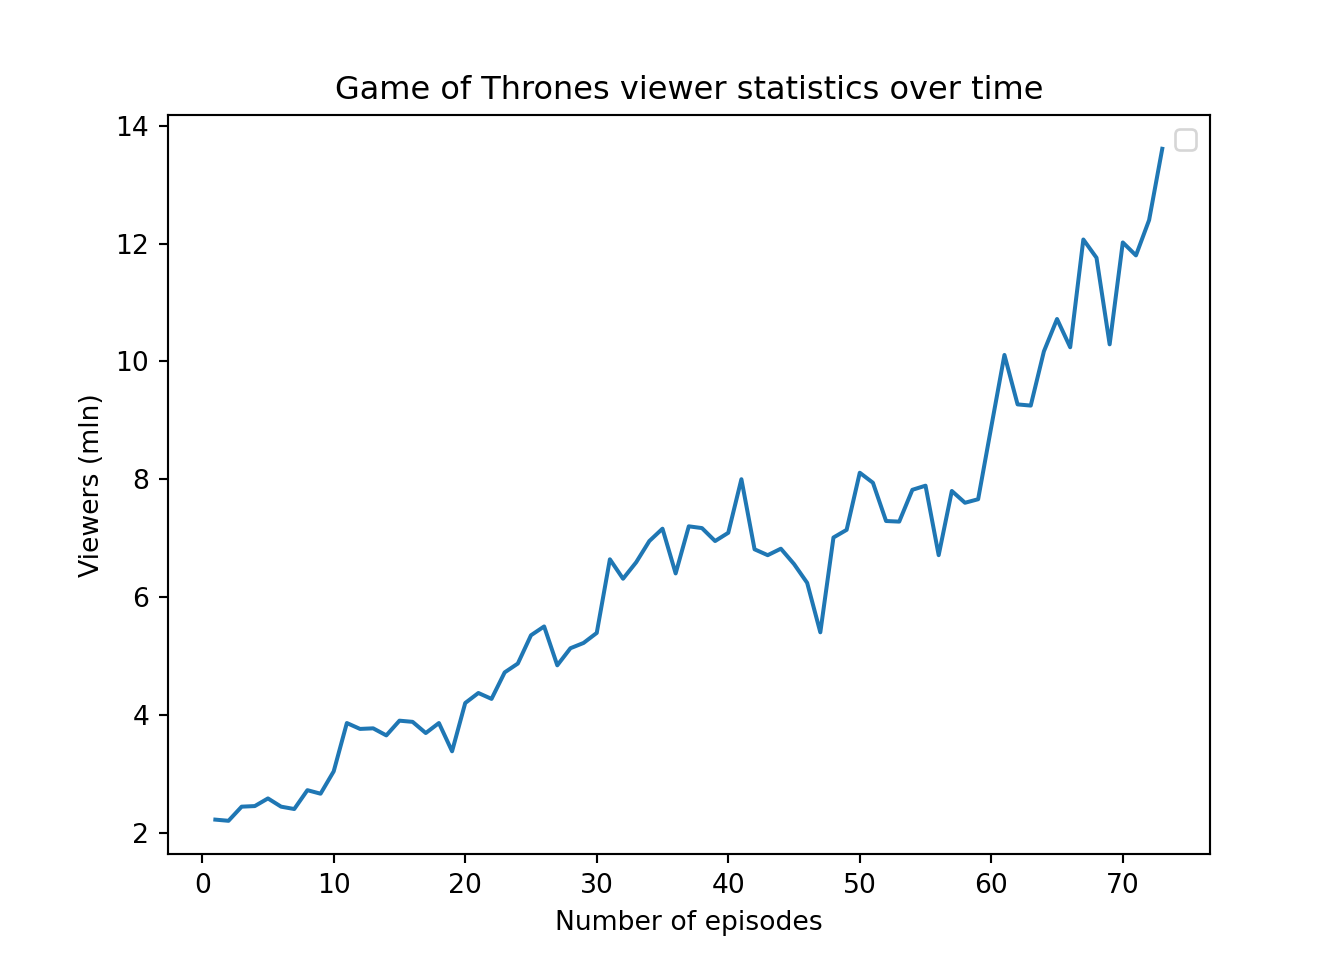
\includegraphics{Rmarkdown_EX2_files/figure-latex/unnamed-chunk-2-1.pdf}

\hypertarget{a-graph-of-season-to-season-changes-in-viewership}{%
\subsubsection{A graph of season-to-season changes in
viewership}\label{a-graph-of-season-to-season-changes-in-viewership}}

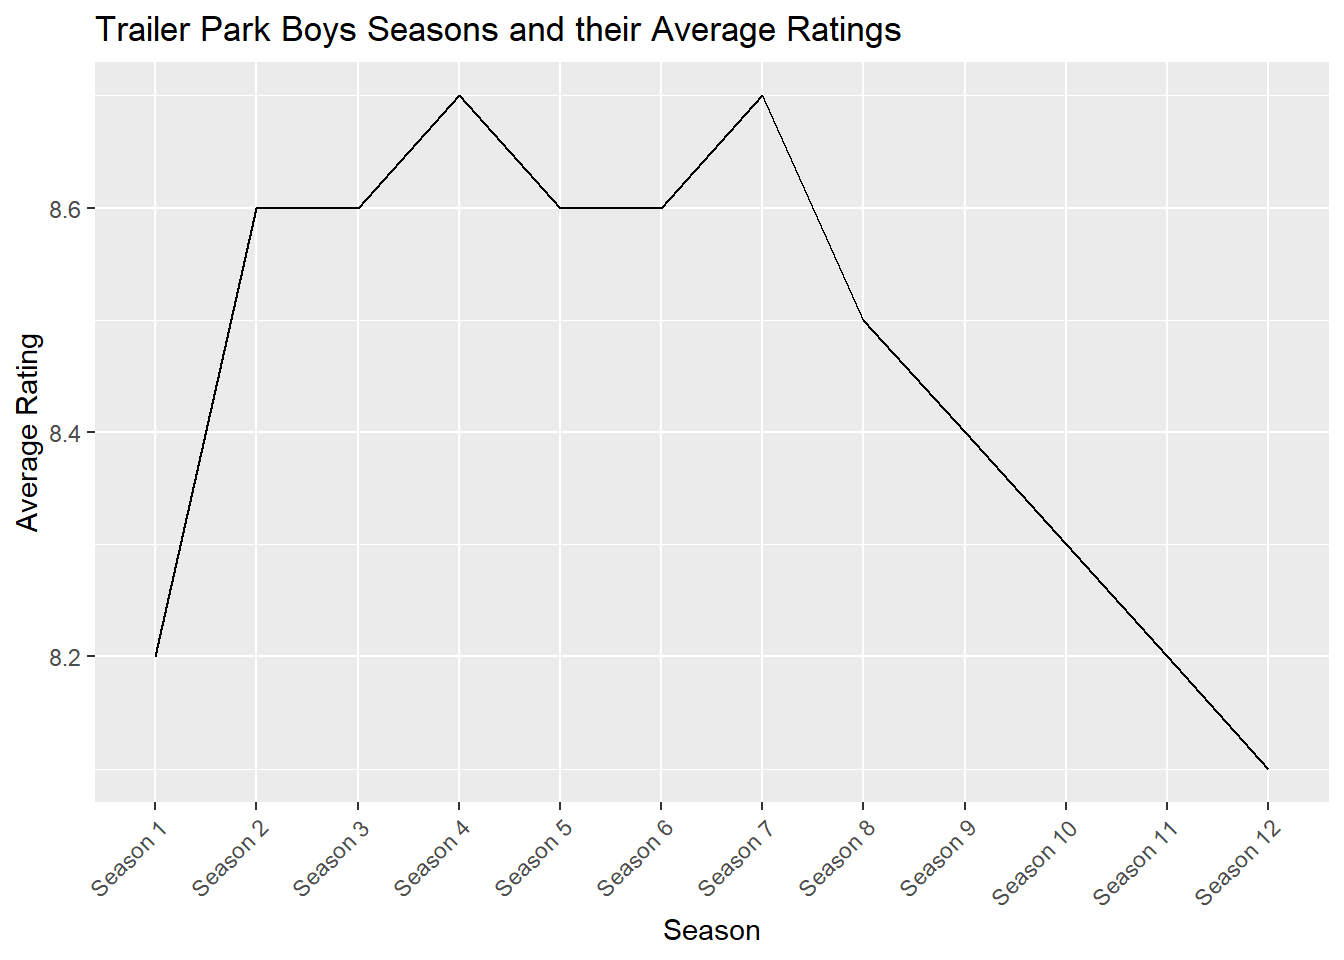
\includegraphics{Rmarkdown_EX2_files/figure-latex/unnamed-chunk-3-1.pdf}

\hypertarget{description-of-the-obseraved-changes}{%
\subsubsection{Description of the obseraved
changes}\label{description-of-the-obseraved-changes}}

Trailer Park Boys had a change in writers and producers after Season 7.
This change could have led to a shift (variable \texttt{avg\_rating}) in
the show's tone or direction, which may not have resonated well with the
audience.

\end{document}
